\documentclass[10pt]{article}
\usepackage[utf8]{inputenc}

\usepackage{graphicx} % Required for inserting images
\usepackage{multicol}
\usepackage{wrapfig}

\usepackage{hyperref}
\usepackage{svg}
\usepackage{subfig}
\usepackage{siunitx}

\usepackage[%
    a4paper,
    top=1.2cm,
    bottom=1.2cm,
    left=2.2cm,
    right=2.2cm,
    marginparwidth=1.75cm
]{geometry}

\title{RS: First Homework}
\author{
    Mark Loboda in Simon Goričar
}
\date{1. 4. 2025}

\begin{document}
\maketitle


\section{Introduction}
In this project, we used the \href{https://www.gem5.org}{\texttt{GEM5}} simulator, an open-source computer-system architecture simulator. It allows users to analyze and test hardware configurations and architectures without actually developing or having to produce any hardware physically. In this report, we're evaluating the performance of the \textit{O3 processor} model using the \textit{Whetstone benchmark} and analyzing the influence of cache size and associativity on the performance of a tiled matrix multiplication program.


\section{Benchmarks}
\subsection{First task: O3 processor}
\subsubsection{The effect of issue width and reorder buffer size on instructions per cycle}
We used the \textit{GEM5} simulator to run the \textit{Whetstone} benchmark on different configurations of the \textit{O3} processor. We performed the benchmark using the combination of the following parameters:

\begin{itemize}
    \item \textbf{Issue Width:} 1, 2, 4, 8
    \item \textbf{Reorder Buffer (ROB) Size:} 2, 4, 8, 16, 32
\end{itemize}

The parameters we configured will likely directly affect how well the processor can exploit instruction-level parallelism (ILP) in out-of-order execution. The \textbf{issue width} is the maximum number of instructions that can be issued in the same cycle. The \textbf{reorder buffer} (ROB) is used to store instructions that have been issued but not yet committed. This allows out-of-order execution while giving the illusion of in-order execution. A larger ROB size gives the processor a larger window for finding independent instructions.

We expect the performance of the \textbf{O3 processor} to increase with \textbf{ROB size} and \textbf{issue width}. When running the benchmark on all the given configurations, we got the following results:

\begin{wrapfigure}{r}{0.65\textwidth}
    \centering
    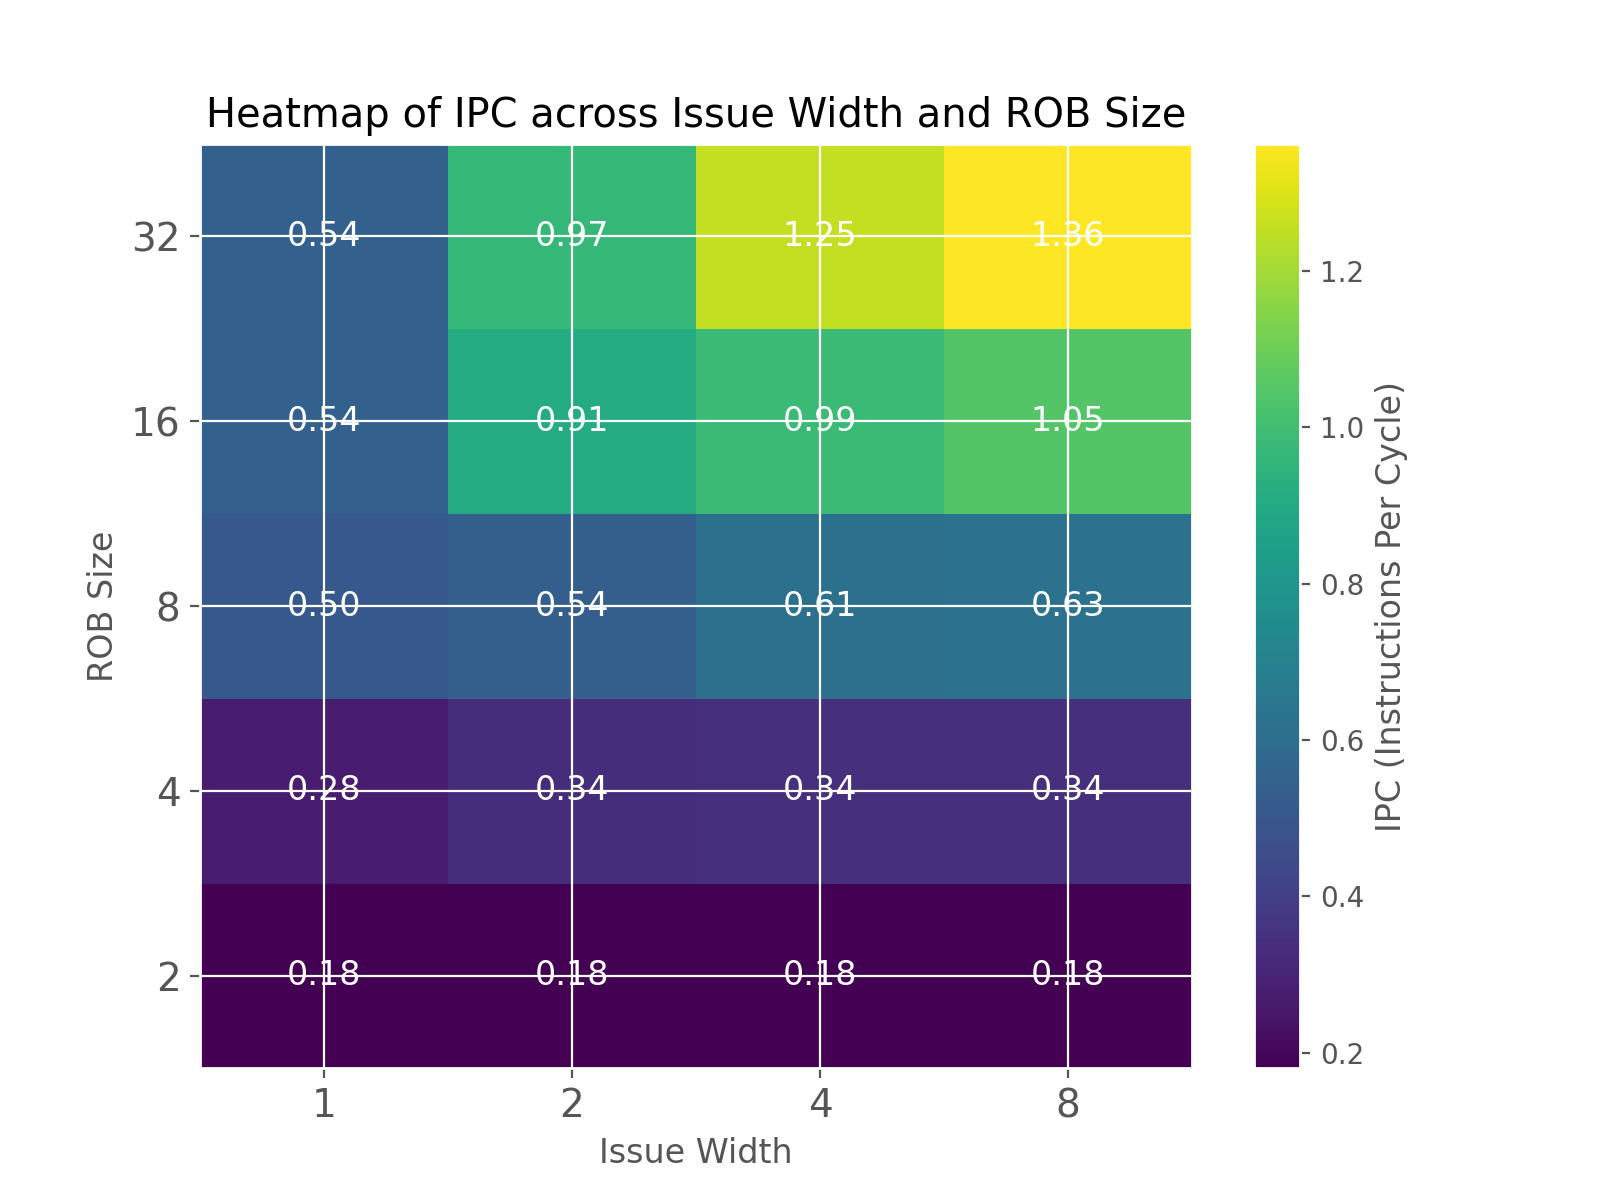
\includegraphics[width=1.0\linewidth]{images/task1/task1_1_ipc_heatmap.png}
    \caption{IPC Heatmap Visualization}
    \label{fig:heatmap}
\end{wrapfigure}

The first thing we notice is that the IPC of the processor increases with issue width and ROB size. We expected this behavior. 

In the runs with a low ROB size of only 2 or 4, we can see that the increase of issue width doesn't provide any gain in performance. We can conclude that the ROB size of less than 2 is extremely restrictive. The processor quickly runs out of space to queue instructions.

When increasing the ROB size from 4 to 8 while keeping the issue width at 1, we can see a substantial gain in IPC. The gain quickly becomes negligible, increasing the ROB size past 8 while leaving the issue width at 1.

We think we can therefore conclude that increasing the issue width without increasing the ROB size doesn't really make a difference at low ROB sizes. After reaching some minimum ROB size, increasing the issue width proves extremely beneficial for the IPC of the processor. The best gain proves to be when $\text{ROB} = 4 \cdot \text{IssueWidth}$.


\subsubsection{The effect of issue width and ROB size on CPI and branch misprediction}
We ran the same \textit{Whetstone} benchmark on the \texttt{GEM5} simulator. We tested two different implementations of branch predictors:

\begin{itemize}
    \item \textbf{Local Branch Predictor (LocalBP)}
    \item \textbf{Multiperspective Perceptron TAGE Predictor (64KB) (TAGE)}
\end{itemize}

Additionally, we tested the predictors using the following two configurations with the goal of testing whether using a different and more complex predictor can increase the performance:

\begin{itemize}
    \item \textbf{Issue Width:} 4, \textbf{ROB size:} 32
    \item \textbf{Issue Width:} 4, \textbf{ROB size:} 64
\end{itemize}

\begin{figure*}[htb!]
    \centering
    \subfloat[]{%
        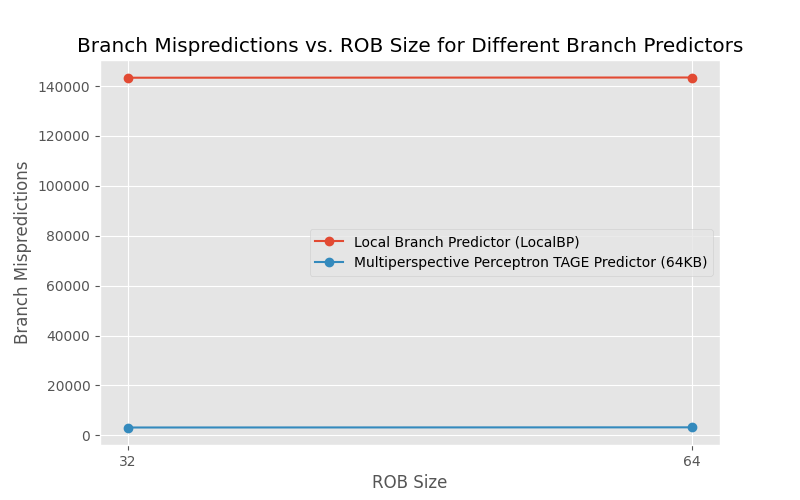
\includegraphics[width=0.49\linewidth]{images/task1/task1_2_branch_mispredictions_vs_rob.png}
        \label{fig:task1:subtask1:ipc}
    }\hfill
    \subfloat[]{%
        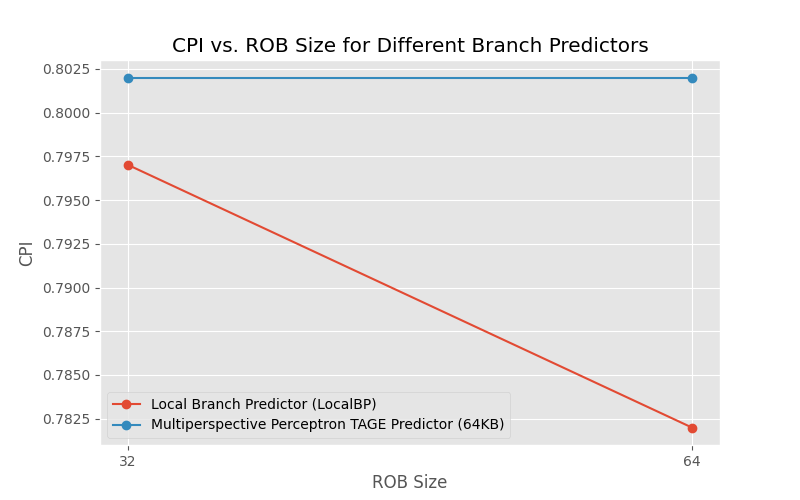
\includegraphics[width=0.49\linewidth]{images/task1/task1_2_cpi_vs_rob.png}
        \label{fig:task1:subtask1:cycles}
    }\\
    \caption{Results of the \textit{Whetstone} benchmark with different branch predictors.}
    \label{fig:task1:subtask2}
\end{figure*}

The branch predictor \textbf{LocalBP} suffers from a very high branch misprediction rate, whereas the \textbf{TAGE} predictor reduces mispredictions by nearly two orders of magnitude. Despite the drastic difference in misprediction counts, CPI remains roughly the same between branch predictor implementations. Doubling the ROB size from 32 to 64 slightly increases the CPI for the LocalBP but yields virtually no change when using the TAGE predictor. The \textit{branch misprediction count} is not affected by the size of the ROB.

The \textbf{TAGE} predictor's higher complexity adds a latency overhead on the prediction, causing the overall CPI to stay roughly the same despite the drastic improvement in \textit{branch misprediction count}. Another reason for the overall CPI staying the same could be a compiler optimization of some parts of the benchmark, where the results are never used (e.g., not printed at the end), therefore not being calculated at all. We would have to check the assembly code of the compiled source code to verify.



\subsection{Second task: cache}
Another benchmark we performed using \texttt{gem5} was one of impact of cache sizes and associativities on instructions per cycle (IPC), L1 miss rate, L2 miss rate, and total cycle count. The workloads we used were three similar matrix multiplication programs, named \texttt{mat\_mult1.c}, \texttt{mat\_mult2.c}, and \texttt{mat\_mult3.c}. The workloads differed only in the order in which they performed matrix multiplication: they used the \texttt{iijjkk}, \texttt{kkiijj}, and \texttt{iikkjj} order, respectively. The matrices were of size $256$ and the block size used for the calculation was $64$.


\subsubsection{Impact of L1 and L2 cache size}
We performed 24 different runs with varying L1 data cache and L2 cache sizes, keeping the set associativity of both caches at 16. The tested L1 data cache sizes were $1~\text{KiB}$, $2~\text{KiB}$, $4~\text{KiB}$, and $8~\text{KiB}$. The tested L2 cache sizes were $32~\text{KiB}$ and $64~\text{KiB}$; all combinations of those L1 and L2 sizes were benchmarked.

We observed practically zero meaningful difference between the three matrix multiplication workloads, at least in the values we measured, so in plots where results aren't shown for all three workloads we'll show only \texttt{mat\_mult1}.


\begin{figure*}[htb!]
    \centering
    \subfloat[Instructions per cycle across L1 and L2 cache sizes.]{%
        \includesvg[width=0.4\linewidth]{images/task2/subtask1/ipc-against-cache_mat_mult1.svg}
        \label{fig:task1:subtask1:ipc}
    }\hfill
    \subfloat[Total cycles across L1 and L2 cache sizes.]{%
        \includesvg[width=0.4\linewidth]{images/task2/subtask1/total-cycles-against-cache_mat_mult1.svg}
        \label{fig:task1:subtask1:cycles}
    }\\
    
    \subfloat[L1 data cache write miss rate using $64~\text{KiB}$ of L2 cache and varying L1 data cache sizes.]{%
        \includesvg[width=0.43\linewidth]{images/task2/subtask1/l1-write-miss-rate-against-l1-size_for-L2-64 KiB.svg}
        \label{fig:task1:subtask1:l1-write}
    }\hfill
    \subfloat[L1 data cache read miss rate using $64~\text{KiB}$ of L2 cache and varying L1 data cache sizes.]{%
        \includesvg[width=0.43\linewidth]{images/task2/subtask1/l1-read-miss-rate-against-l1-size_for-L2-64 KiB.svg}
        \label{fig:task1:subtask1:l1-read}
    }\\

    \caption{IPC, cycle count, and L1 results of our cache benchmark.}
    \label{fig:task1:subtask1}
\end{figure*}

\begin{figure*}[htb!]
    \centering
    \subfloat[L2 cache miss rate when using an L1 data cache of size $1~\text{KiB}$]{%
        \includesvg[width=0.4\linewidth]{images/task2/subtask1/l2-miss-rate-against-l2-size_for-L1-1 KiB.svg}
        \label{fig:task1:subtask1:l2:l1-1}
    }\hfill
    \subfloat[L2 cache miss rate when using an L1 data cache of size $2~\text{KiB}$]{%
        \includesvg[width=0.4\linewidth]{images/task2/subtask1/l2-miss-rate-against-l2-size_for-L1-2 KiB.svg}
        \label{fig:task1:subtask1:l2:l1-2}
    }\\
    
    \subfloat[L2 cache miss rate when using an L1 data cache of size $4~\text{KiB}$]{%
        \includesvg[width=0.4\linewidth]{images/task2/subtask1/l2-miss-rate-against-l2-size_for-L1-4 KiB.svg}
        \label{fig:task1:subtask1:l2:l1-4}
    }\hfill
    \subfloat[L2 cache miss rate when using an L1 data cache of size $8~\text{KiB}$]{%
        \includesvg[width=0.4\linewidth]{images/task2/subtask1/l2-miss-rate-against-l2-size_for-L1-8 KiB.svg}
        \label{fig:task1:subtask1:l2:l1-8}
    }\\

    \caption{L2 results of our cache benchmark.}
    \label{fig:task1:subtask1:l2}
\end{figure*}

First off, let's have a look at the changes in \textbf{instructions per cycle} (figure \ref{fig:task1:subtask1:ipc}).
As we can see on the plot, we L2 cache size had essentially zero impact on the overall IPC, while increasing the L1 data cache size had some nearly negligible impact using small sizes, but jumped considerably when set to $8~\text{KiB}$. For context, the size of each of the three matrices used in the workload is $256~\text{KiB}$, so it is possible that, when using $8~\text{KiB}$, the reduced miss rate is finally large enough to fit a large chunk of the matrices into L1, and therefore results in significantly less waiting for the cache, in turn raising the IPC value. The L2 cache size doesn't seem to impact the average IPC.

Secondly, \textbf{total cycles} (figure \ref{fig:task1:subtask1:cycles}). 
The results mirror the improvements seen in the instruction per cycle plot: as the IPC increases, the total cycle count decreases, as we'd expect. As before, the L2 cache size doesn't seem to impact total cycles (nor IPC); it seems the L2 misses are too rare to show up.

Thirdly, \textbf{L1 miss rate} (figures \ref{fig:task1:subtask1:l1-read} and \ref{fig:task1:subtask1:l1-write}). 
In the read miss rate plot, a similar jump can be observed as with the IPC value. However, the write miss rate shows a much more gradual decrease over the L1 data cache size from $1~\text{KiB}$ to $8~\text{KiB}$. Our reasoning is that writes are only done into a single matrix, while reads are done from three (A, B, and the destination matrix). We think this causes the write misses to be more easily optimizable by increasing the L1 size, because the destination matrix likely isn't competing for cache as heavily as the two source matrices.

Lastly, \textbf{L2 miss rate} (figure \ref{fig:task1:subtask1:l2}).
Here we see a similar pattern as with the L1 miss rate plot, just in reverse.
Interestingly, unless L1 is very large, L2 size doesn't seem to actually impact L2 miss rate. As L1 increases to $8~\text{KiB}$, we see the same jump we saw in the L1 data cache read miss rate. At that L1 size, we even see the first impact of L2 and matrix multiplication strategy choices: an increased L2 size actually improves the L2 miss rate, and we can notice a small change in performance of different matrix multiplication implementations --- the \texttt{iijjkk} order seemingly performing the worst --- though we don't think the results provide a clear enough distinction to warrant a conclusion. What we should take away from this is more of a confirmation of the jump we saw in the L1 read miss rate graph: as L1 reads start missing less frequently, the L2 cache gets used more and more, warranting more cache misses, and the increased L2 size finally making an impact.



\subsubsection{Impact of L1 and L2 associativity}
The second cache benchmark we performed was with a fixed L1 data cache of size $4~\text{KiB}$ and a fixed L2 size of $256~\text{KiB}$, while varying the cache associativities across $1$, $2$, $4$, $8$, and $16$. As such, we performed 75 runs with different combinations of these parameters and while running all three workloads.

Once again, we observed a minimal, if any, difference between the three matrix multiplication workloads, so once again, we'll show only \texttt{mat\_mult1} in the plots.

\begin{figure*}[htb!]
    \centering
    
    \subfloat[Total cycle count across cache associativity combinations.]{%
        \includesvg[width=0.4\linewidth]{images/task2/subtask2/total-cycles-across-2d-cache-associativities_mat_mult1.svg}
        \label{fig:task1:subtask2:main:totalcycles}
    }\hfill
    \subfloat[L2 cache miss rate across cache associativity combinations.]{%
        \includesvg[width=0.4\linewidth]{images/task2/subtask2/l2-miss-rate-across-2d-cache-associativities_mat_mult1.svg}
        \label{fig:task1:subtask2:main:l2-miss}
    }\\
    
    \subfloat[IPC across cache associativity combinations.]{%
        \includesvg[width=0.6\linewidth]{images/task2/subtask2/ipc-across-2d-cache-associativities_mat_mult1.svg}
        \label{fig:task1:subtask2:main:ipc}
    }

    \caption{Total cycles, L2, and IPC results of our cache associativity benchmark.}
    \label{fig:task1:subtask2:main}
\end{figure*}

\begin{figure*}[htb!]
    \centering
    \subfloat[L1 read miss rate across cache associativity combinations.]{%
        \includesvg[width=0.42\linewidth]{images/task2/subtask2/l1-read-miss-rate-across-2d-cache-associativities_mat_mult1.svg}
        \label{fig:task1:subtask2:l1:read}
    }\hfill
    \subfloat[L1 write miss rate across cache associativity combinations.]{%
        \includesvg[width=0.42\linewidth]{images/task2/subtask2/l1-write-miss-rate-across-2d-cache-associativities_mat_mult1.svg}
        \label{fig:task1:subtask2:l1:write}
    }

    \caption{L1 miss rate results of our cache associativity benchmark.}
    \label{fig:task1:subtask2:l1}
\end{figure*}

First off, let's look at how \textbf{IPC} and \textbf{total cycles} are impacted.
As we can see in figures \ref{fig:task1:subtask2:main:ipc} and \ref{fig:task1:subtask2:main:totalcycles}, both IPC and total cycles benefit positively from an increase in both L1 and L2 cache associativity, though the improvements fall off at a certain point; for example, note how --- at least for our workload --- the optimal IPC was achieved with the combination of 2-way associative L1 cache and 4-way-or-more associative L2 cache. The same is true for the total cycle count. We think a different pattern would emerge under a different --- perhaps more allocation-heavy --- workload.

Secondly, \textbf{L1 read and write miss rates} (figures \ref{fig:task1:subtask2:l1:read} and \ref{fig:task1:subtask2:l1:write}) can be seen to be somewhat decreasing as L1 cache associativity is increased. For read misses, this is only true up to 2-way associativity, after which the miss rates rise up to nearly the initial rate again. For write misses, it is evident that higher associativity is better, with no apparent downside.

Lastly, \textbf{L2 miss rate} (figure \ref{fig:task1:subtask2:main:l2-miss}) seems to be influenced primarily by an increase in L2 associativity. However, due to L1 being in front of L2 and taking some misses, we can see a very slight improvement as L1 associativity is increased as well and the underlying L1 miss rate falls.


\end{document}
